\documentclass[11pt,ngerman]{article}
\usepackage{geometry}
\usepackage[T1]{fontenc}
\usepackage[utf8]{inputenc}
\usepackage{babel}
\usepackage{lmodern}%get scalable font
\usepackage{titling}
\usepackage{relsize}
\usepackage{biblatex}
\usepackage{hyperref}
\usepackage{paralist}
\usepackage[table, dvipsnames]{xcolor}
\usepackage{booktabs}
\usepackage{setspace}
\usepackage{float}
\usepackage{graphicx}
\usepackage{listings}
\usepackage[most]{tcolorbox}
\usepackage{titlesec}

% Link colors
\hypersetup{
    colorlinks,
    linkcolor={blue},
    citecolor={red},
    urlcolor={blue}
}

% inline code macro
\definecolor{lightgray}{gray}{0.9}
\lstset{
    showstringspaces=false,
    basicstyle=\ttfamily,
    keywordstyle=\color{blue},
    commentstyle=\color[grey]{0.6},
    stringstyle=\color[RGB]{255,150,75}
}
\newcommand{\inlinecode}[2]{\colorbox{lightgray}{\lstinline[language=#1]$#2$}}

% Code block settings
\definecolor{codegreen}{rgb}{0,0.6,0}
\definecolor{codegray}{rgb}{0.5,0.5,0.5}
\definecolor{codepurple}{rgb}{0.58,0,0.82}
\definecolor{backcolour}{rgb}{0.95,0.95,0.92}

\lstdefinestyle{mystyle}{
    backgroundcolor=\color{backcolour},
    commentstyle=\color{codegreen},
    keywordstyle=\color{magenta},
    numberstyle=\tiny\color{codegray},
    stringstyle=\color{codepurple},
    basicstyle=\ttfamily\footnotesize,
    breakatwhitespace=false,
    breaklines=true,
    captionpos=b,
    keepspaces=true,
    numbers=left,
    numbersep=5pt,
    showspaces=false,
    showstringspaces=false,
    showtabs=false,
    tabsize=2
}
\lstset{style=mystyle}

% double quotes macro
% usage: \quotes{arg1}  => in text: "arg1"
\newcommand{\quotes}[1]{``#1''}

% paragraph as subsubsubsection
\setcounter{secnumdepth}{4}
\titleformat{\paragraph}
{\normalfont\normalsize\bfseries}{\theparagraph}{1em}{}
\titlespacing*{\paragraph}
{0pt}{3.25ex plus 1ex minus .2ex}{1.5ex plus .2ex}

\geometry{a4paper, top=25mm, left=25mm, right=25mm, bottom=20mm,
    headsep=10mm, footskip=12mm}

\renewcommand{\arraystretch}{1.5}

\pretitle{\begin{center}\linespread{1.5}\huge}
    \posttitle{\par\end{center}\vspace{0.5em}}

\begin{document}

    \title{SWEN1\\Praktikum 06 IoT\\
        \vspace{1cm}
        \small{ZHAW  School of Engineering\\Klasse: IT18tb\_zh}
        \vspace{1.5cm}
    }
    \author{
        Huber, Patrick\\
        \small{huberpa4@students.zhaw.ch}
        \vspace{1.5cm}
    }
   \date{\today}

    \maketitle
    \newpage

    \tableofcontents
    \listoffigures
%    \lstlistoflistings
    \newpage

    \section{Praktikum IoT}

    \subsection{Aufgabe 1 - Domänenmodell und Anwendungsfälle}
    \label{ssec:Aufg1}

    \subsubsection{Domänenmodell}
    In \autoref{fig:DM_Aufg1} ist eine mögliche Lösung für das Domänenmodell abgebildet:
    \begin{figure}[H]
        \centering
        \makebox[\textwidth][c]{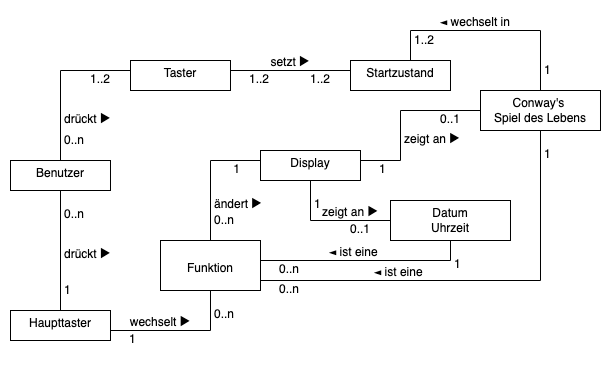
\includegraphics[width=1\textwidth]{figures/SWEN1_Prkt6_IoT_DM.png}}
        \caption{UML Domänenmodell - IoT Display}
        \label{fig:DM_Aufg1}
    \end{figure}

    \subsubsection{Anwendungsfälle}
    \label{sssec:Anwendungsfälle}
    Die IoT Anwendung könnte mit den folgenden zwei Anwendungsfällen beschrieben werden:
    \begin{itemize}
        \item  \hyperref[p:UC1datetime]{UC1: Datum und Uhrzeit anzeigen - \quotes{casual}}
        \item\hyperref[p:UC2Spielspielen]{UC2: Conway's Spiel des Lebens spielen - \quotes{casual}}
    \end{itemize}

    \paragraph{UC1: Datum und Uhrzeit anzeigen - \quotes{casual}}
    \label{p:UC1datetime}
    \begin{tcolorbox}[enhanced, breakable, sharp corners, width=\dimexpr\textwidth-15mm\relax ,enlarge left by=10mm ,fontupper=\linespread{1.1}\selectfont, boxrule=1pt, title={UC1: Datum und Uhrzeit anzeigen}, colback=white, colframe=gray!22, coltitle=black]
         \textit{Standardszenario:} \newline
         Der Benutzer drückt wiederholt den Haupttaster \quotes{\textit{main}}, bis das Display \textbf{Datum und Uhrzeit} anzeigt. \newline
        \newline
        \textit{Alternatives Szenario:} \newline
        Der Benutzer muss den Haupttaster \quotes{\textit{main}} nicht drücken, da \textbf{Datum und Uhrzeit} bereits ersichtlich sind.
    \end{tcolorbox}

    \paragraph{UC2: Conway's Spiel des Lebens spielen - \quotes{casual}}
    \label{p:UC2Spielspielen}
    \begin{tcolorbox}[enhanced, breakable, sharp corners, width=\dimexpr\textwidth-15mm\relax ,enlarge left by=10mm ,fontupper=\linespread{1.1}\selectfont, boxrule=1pt, title={UC2: Conway's Spiel des Lebens spielen}, colback=white, colframe=gray!22, coltitle=black]
        \textit{Standardszenario:} \newline
        Der Benutzer drückt wiederholt den Haupttaster \quotes{\textit{main}}, bis das Display \textbf{Conway's Spiel des Lebens} anzeigt. Das Spiel kann nun weitergespielt werden.\newline
        \newline
        \textit{Alternative Szenarios:} \newline
        Der Benutzer muss den Haupttaster \quotes{\textit{main}} nicht drücken, da \textbf{Conway's Spiel des Lebens} bereits ersichtlich sind. \newline
        \newline
        \textbf{Conway's Spiel des Lebens} wird angezeigt und der Benutzer drückt zusätzlich den \textit{blauen} Taster für einen neuen Startzustand. \newline
         \newline
         \textbf{Conway's Spiel des Lebens} wird angezeigt und der Benutzer drückt zusätzlich den \textit{grünen} Taster für einen neuen interessanten Startzustand. \newline\newline
    \end{tcolorbox}

    \subsection{Aufgabe 2 - Zustandsdiagramm \quotes{Conway's Spiel des Lebens}}
    \label{ssec:Aufg2}

    \subsubsection{Zustandsdiagramm}
    \label{sssec:Zustandsdiagramm}
    Zustandsdiagramm \quotes{Conway's Spiel des Lebens}
    \begin{figure}[H]
        \centering
        \makebox[\textwidth][c]{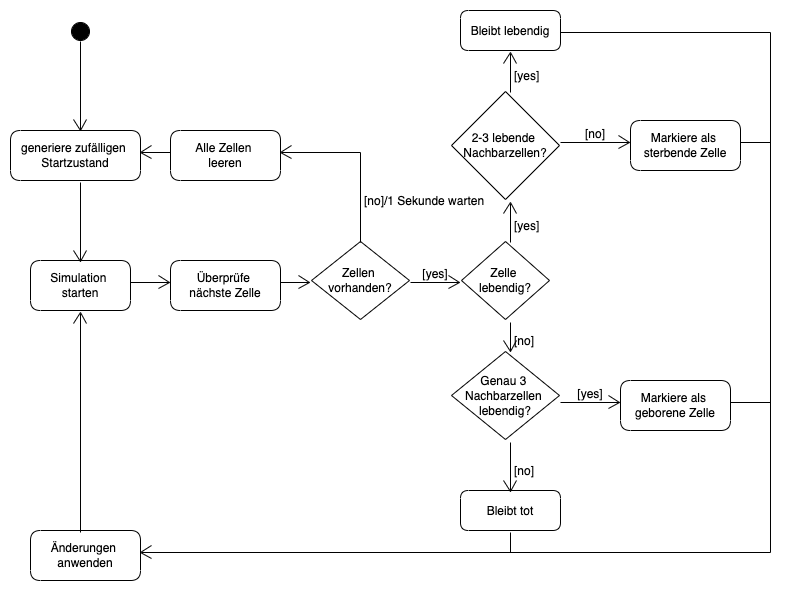
\includegraphics[width=1\textwidth]{figures/SWEN1_IoT_Zustandsdiagramm.png}}
        \caption{UML Zustandsdiagramm - \quotes{Conway's Spiel des Lebens}}
        \label{fig:ZD_Aufg2}
    \end{figure}

    \newpage
    \subsection{Aufgabe 3 - Design}
    \label{ssec:Aufg3}
    Eine mögliches übergeordnetes Design für die Umsetzung der  IoT Anwendung :
    \begin{itemize}
        \item  MVC-Pattern der Applikationssegmente, bestehend aus Clock- bzw. Game-Model, -View, -Controller.
        \item Composite-Pattern für die Ansichten inklusive \inlinecode{Java}{ButtonStrategy} und die \inlinecode{Java}{EventListener} (Timer, Click, etc.).
        \item Strategy-Pattern für Datum und Uhrzeit mit der \inlinecode{Java}{FetchStrategy}.
    \end{itemize}
    Es fehlt noch das Plattform-Objekt und der Main-Button.

    \begin{figure}[H]
        \centering
        \makebox[\textwidth][c]{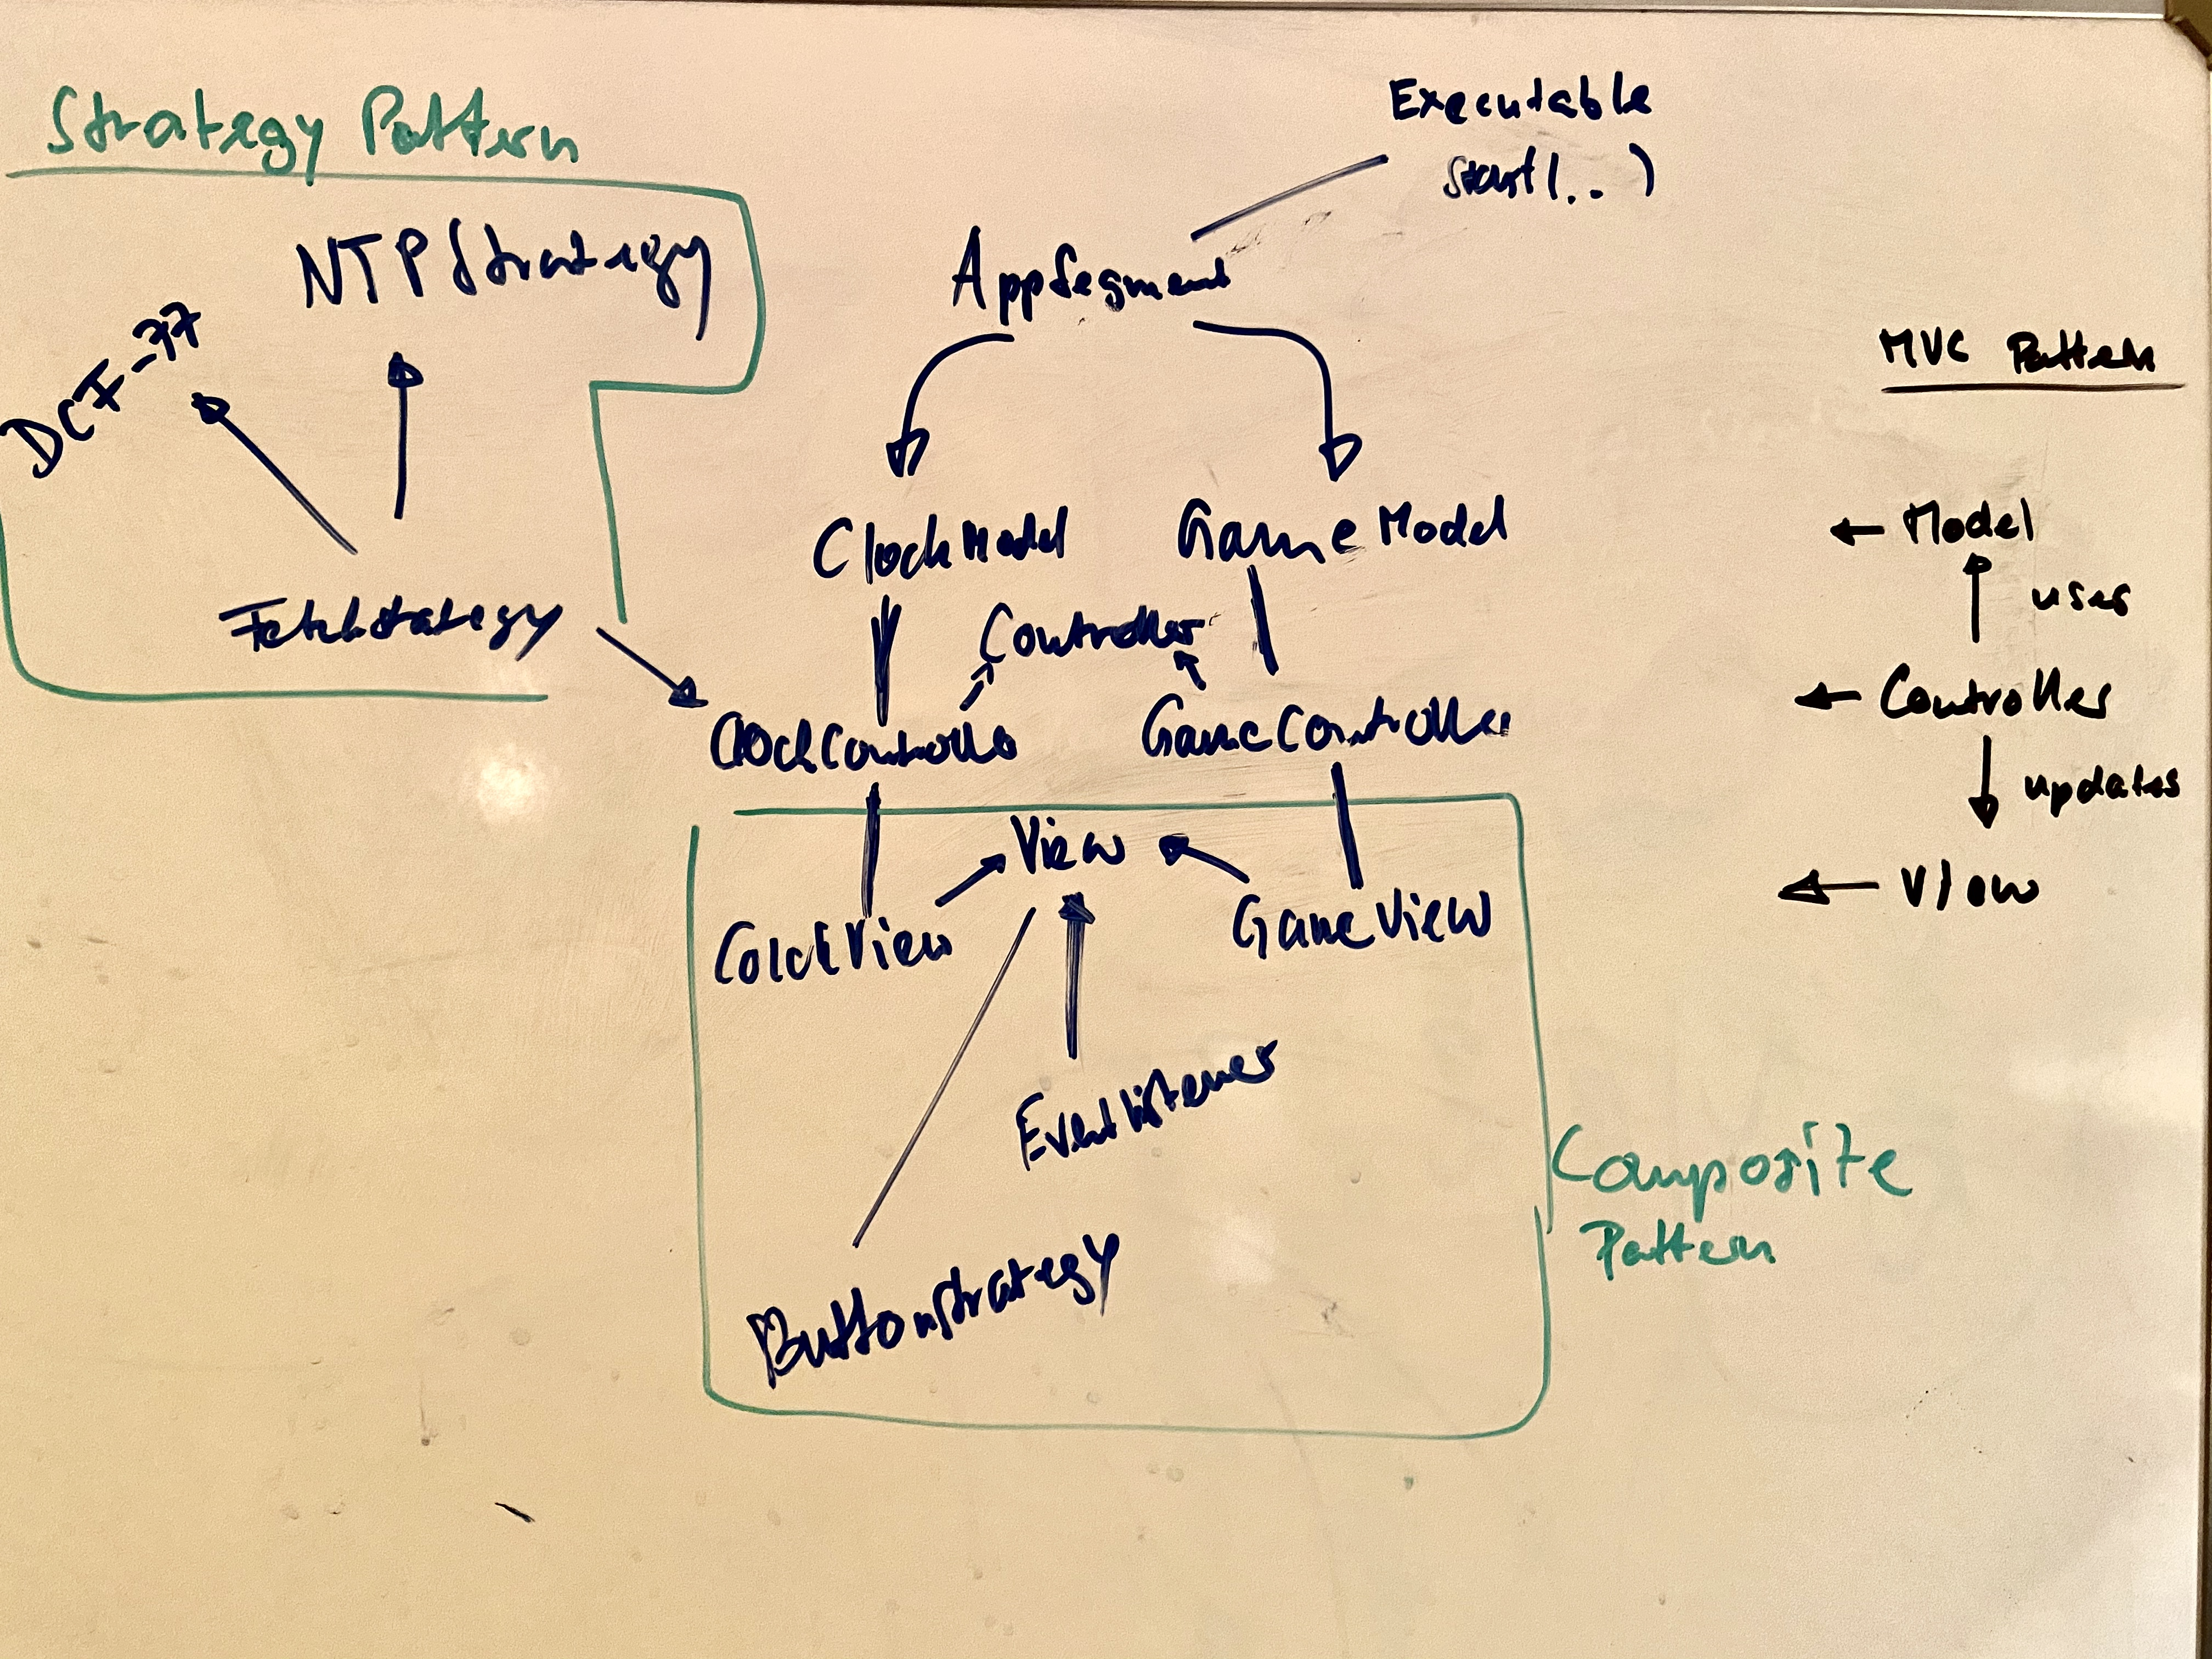
\includegraphics[width=1\textwidth]{figures/IoT_Design.jpg}}
        \caption{Übergeordnetes Design der IoT Anwendung als grobe Skizze}
        \label{fig:DesignSkizze_Aufg3}
    \end{figure}

    \newpage
    \subsection{Aufgabe 4 - Domänenlogik Uhr}
    \label{ssec:Aufg4}
    Skizze abstrakte Domänenlogik für Datum und Uhrzeit:

    \begin{figure}[H]
        \centering
        \makebox[\textwidth][c]{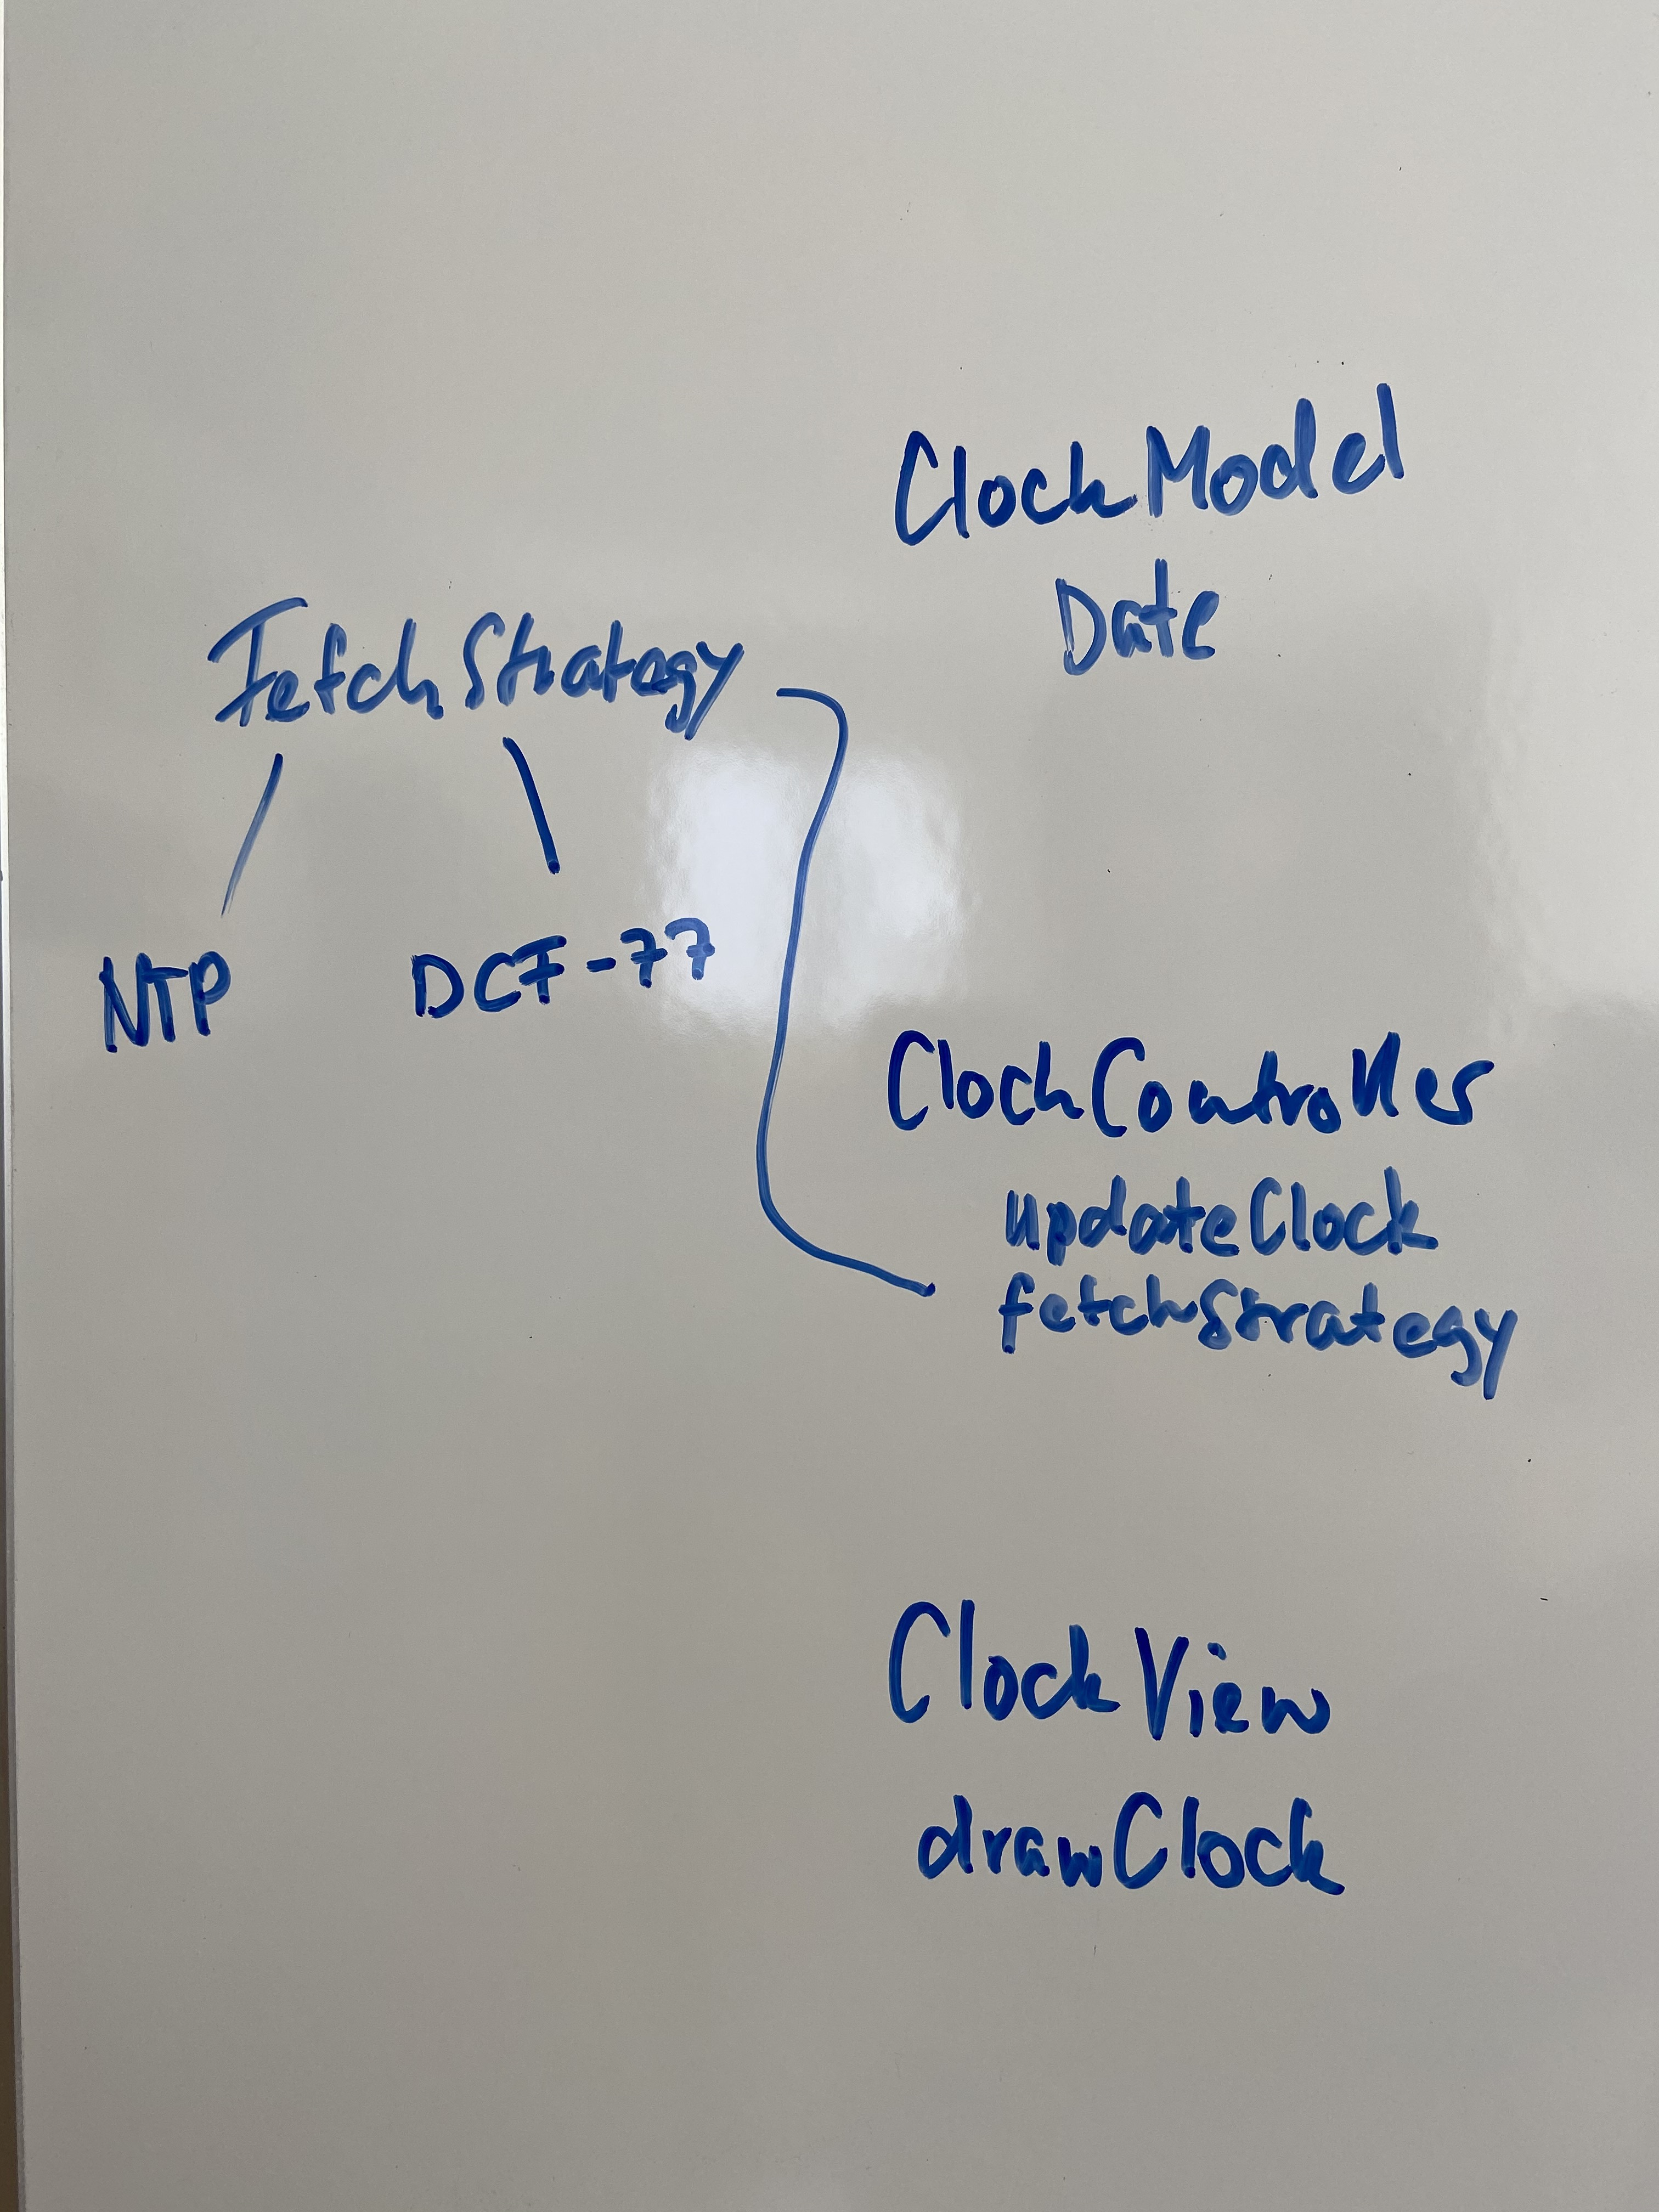
\includegraphics[width=0.75\textwidth]{figures/IoT_KD_Clock.jpg}}
        \caption{Abstrakter Entwurf Domänenlogik für die Uhr}
        \label{fig:KD_Aufg4}
    \end{figure}

    \newpage
    \subsection{Aufgabe 5 - Domänenlogik Spiel}
    \label{ssec:Aufg4}
    Skizze abstrakte Domänenlogik für das Spiel:

    \begin{figure}[H]
        \centering
        \makebox[\textwidth][c]{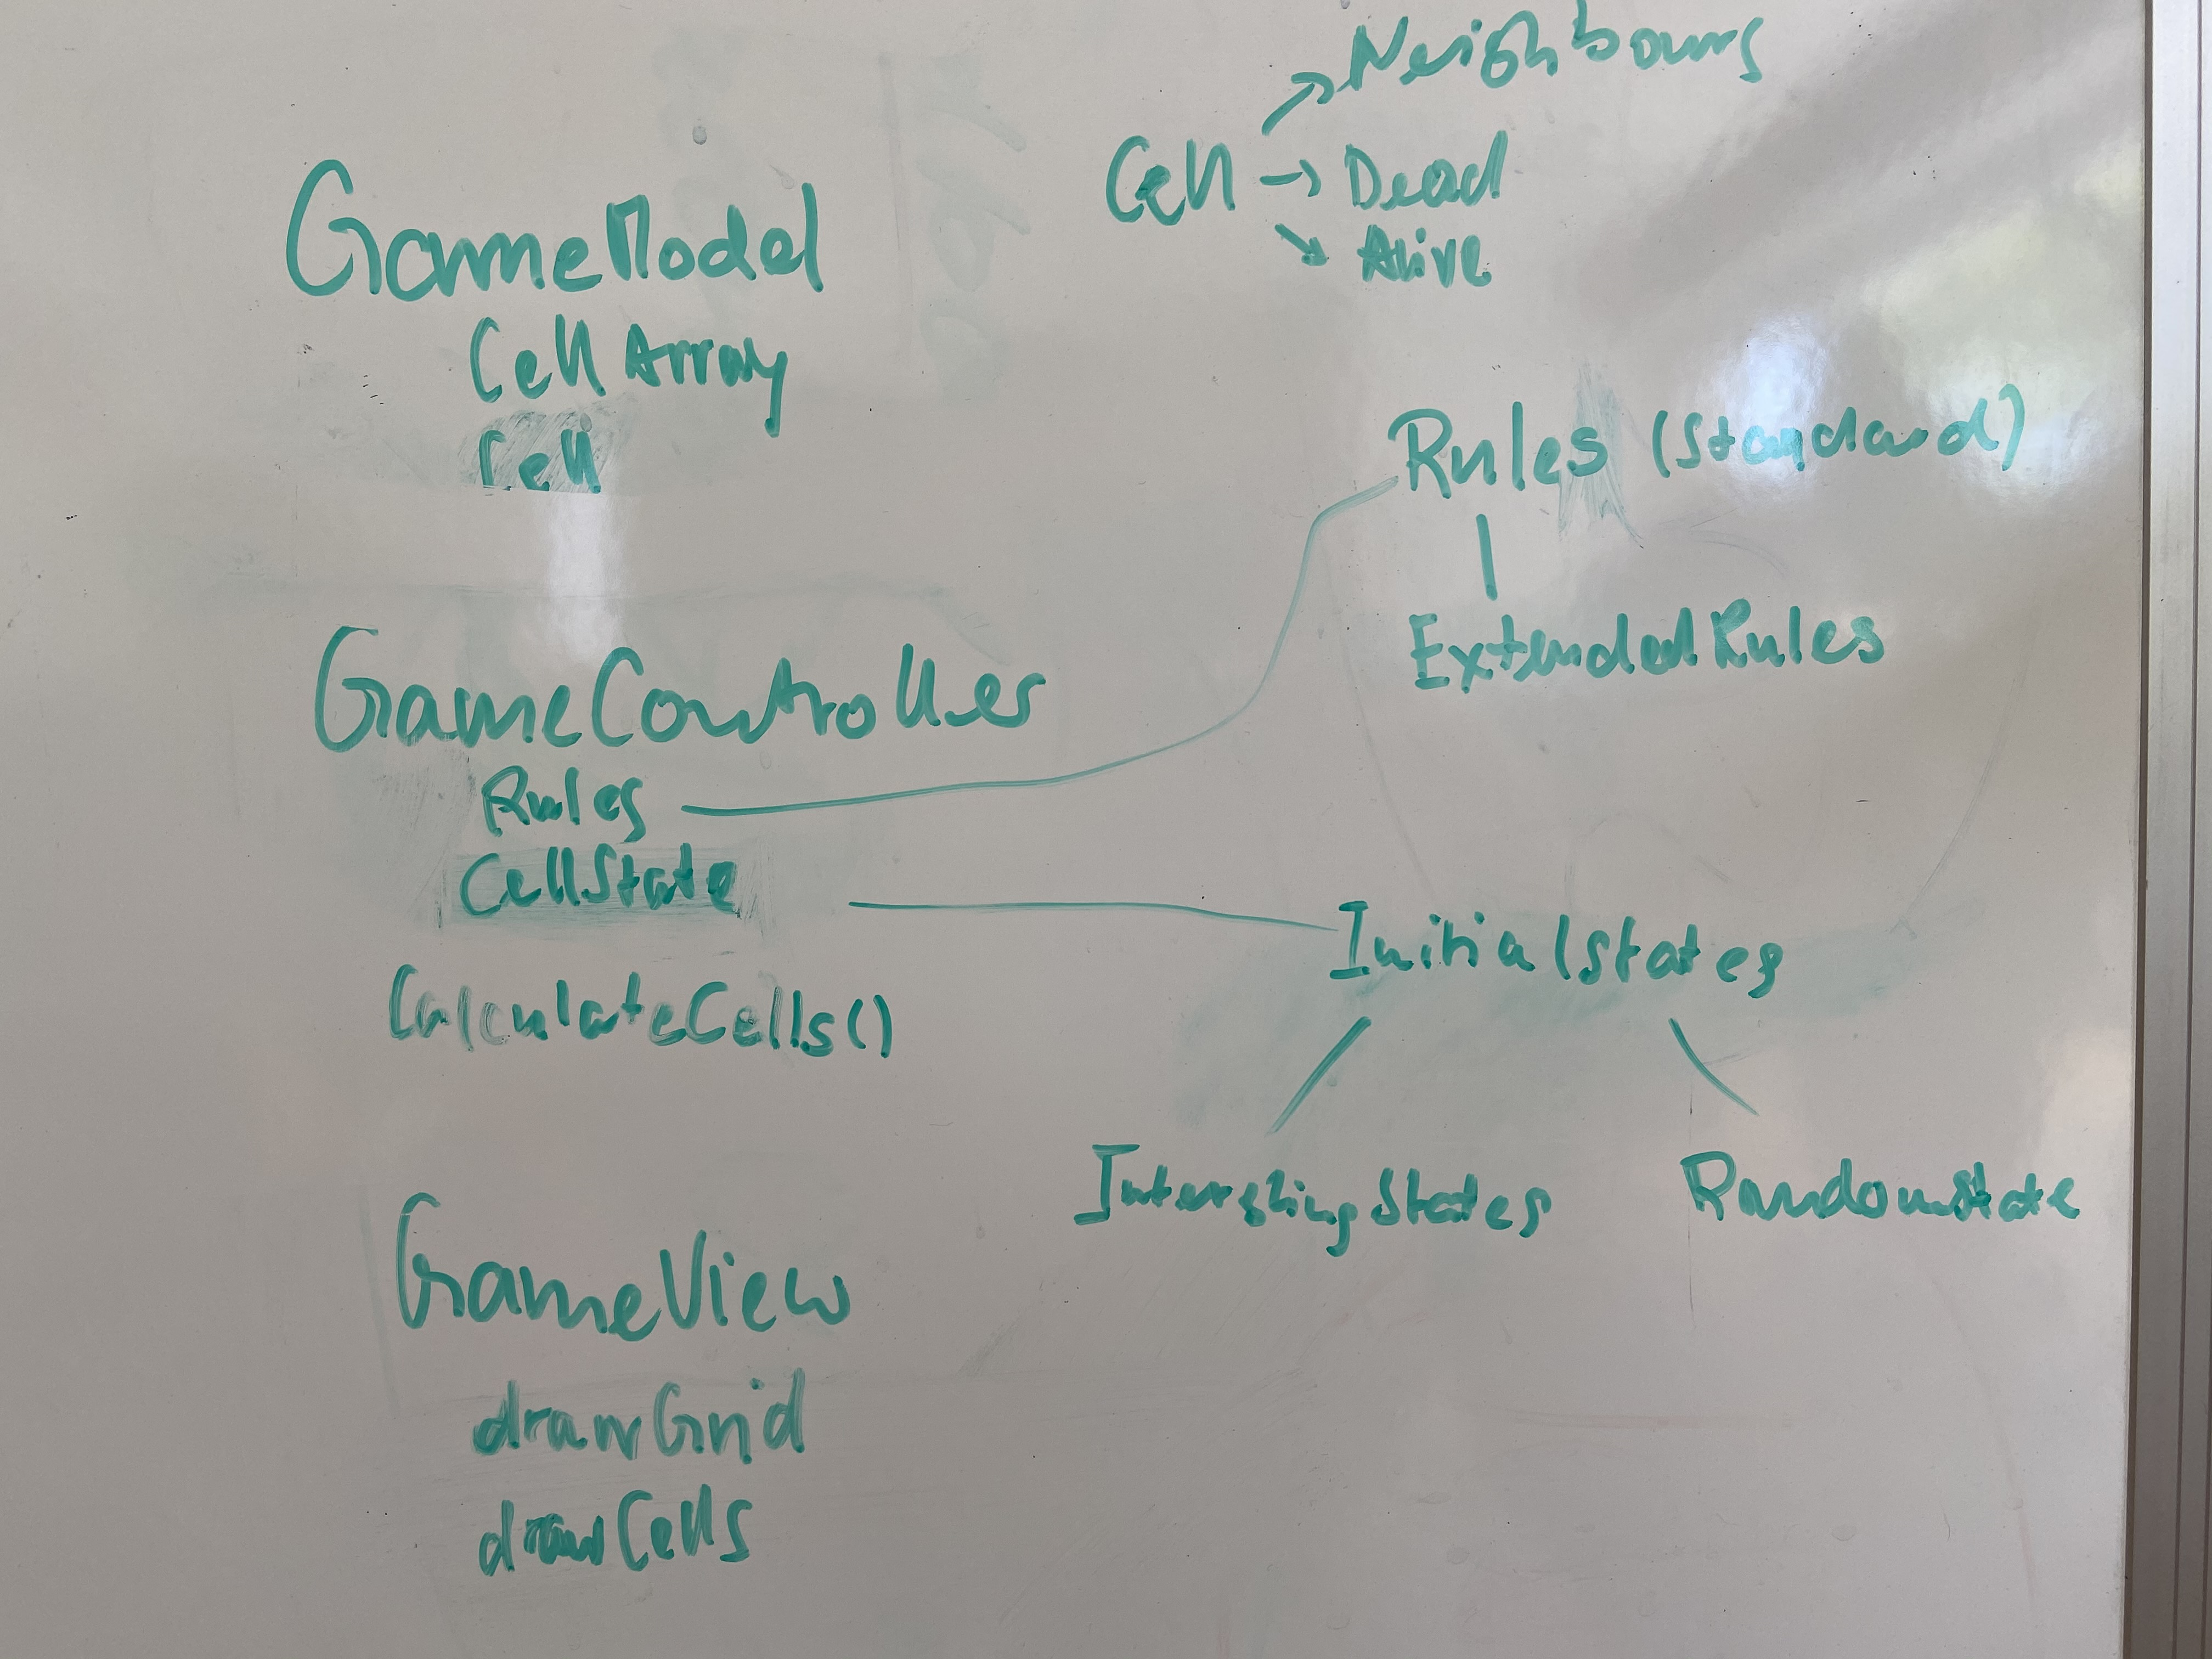
\includegraphics[width=1\textwidth]{figures/IoT_KD_Game.jpg}}
        \caption{Abstrakter Entwurf Domänenlogik für das Spiel}
        \label{fig:KD_Aufg4}
    \end{figure}

\end{document}

